\documentclass[runningheads,envcountsect,envcountsame]{lncs/llncs}
% \usepackage[a4paper,textwidth=12.6cm,textheight=20.5cm,heightrounded,hratio=1:1,vratio=3:5]{geometry}
\usepackage[table]{xcolor} 
\usepackage{fontspec}
\usepackage{luatexbase}
\usepackage{microtype}
\usepackage{textcomp}
\usepackage{graphicx}
\usepackage[bookmarksdepth=2,pdfauthor={Daniel Petri, Roy Hermanns, Haikun Huang},pdfsubject={A Petri Net Modeling and Testing Language Developed with MontiCore}]{hyperref}
\pdfvariable minorversion=7

\usepackage{listings}
\usepackage{xcolor}
\renewcommand\UrlFont{\color{blue}\rmfamily}
\usepackage{float}
\usepackage{array}

\newfloat{lstfloat}{htb}{lop}
\floatname{lstfloat}{Listing}
\def\lstfloatautorefname{Listing}

\lstdefinestyle{petrinet}{
    keywordstyle=[2]{\color{blue}\bfseries},
    otherkeywords={<-,->},
    morekeywords={petrinet,assert,place,transition,initial},
    morekeywords=[2]{<-,->}
}
\lstdefinestyle{mcgrammar}{
    morekeywords={grammar,extends,scope,interface,astrule,method,enum,implements,symbol,abstract}
}
\lstset{frame=single,numbers=left,basicstyle=\scriptsize,literate={"}{\textquotedbl}1,escapeinside={/@}{@/}}

\usepackage{amsmath}
\usepackage{amsfonts}
\usepackage{amssymb}

\usepackage{subcaption}

\usepackage{tikz}
\usetikzlibrary{arrows,shapes,snakes,automata,backgrounds,petri,positioning}
\tikzset{node distance=1.3cm,>=stealth',bend angle=45,auto}
\tikzstyle{place}=[circle,thick,draw=blue!75,fill=blue!20,minimum size=6mm]
\tikzstyle{transition}=[rectangle,thick,draw=black!75,
fill=black!20,minimum width=8mm,inner ysep=2pt]
\tikzstyle{treenode}=[rectangle,thick,draw=blue!75,fill=blue!20,minimum size=6mm]

\usepackage{tikz-uml}

\usepackage{multirow}
\usepackage[flushleft]{threeparttable}

\newcommand\rdot{{}^\bullet}

\hyphenation{co-ve-ra-bi-li-ty}

\begin{document}

\title{\emph{Petrinets Testing}: A Petri Net Modeling and Testing Language Developed with MontiCore\thanks{Practical Project for the lecture ``Software Language Engineering'' by Prof.\ Dr.\ B.\ Rumpe. The authors are grateful to Imke Drave for her supervision of the project.}}
\titlerunning{\emph{Petrinets Testing}: Petri Net Testing with MontiCore}

\author{Daniel Petri \and
Roy Hermanns \and
Haikun Huang}
\authorrunning{D. Petri, R. Hermanns, H. Huang}
\institute{
RWTH Aachen University, Aachen, Germany \\
\email{\{daniel.petri, roy.hermanns, haikun.huang\}@rwth-aachen.de}
}

\maketitle

% TeX root = ../../paper.tex

\begin{abstract}

    Ensuring reliability and security of software to improve the quality becomes an urgent issue. Petri nets are not only a graphical modeling tool but also a formal method with strict grammar and semantic definitions that can be used to model and describe the system effectively at the same time. Therefore model-based testing techniques with petri net can be used to develop tests of systems based on formal criteria to find errors at early stages in development. It is even possible to generate testcases automatically.
    
    We define a textual modeling language, \emph{Petrinets Testing}, based on the MontiCore Language Workbench \cite{monticore2020}. Our language is an extension of the \emph{petrinets4analysis} language, which is to analyze the given petri net model. The goal of the \emph{Petrinets Testing} language is to verify the correctness of the given petri net model. Due to the powerful language generation by MontiCore based on a simple context-free grammar, only a small hand-written codebase is needed, enhancing maintainability and extensibility.
    
    Our work is to create a modeling DSL (domain specific language) using the Monticore to automate the inspection process for petri nets. Moreover, The test cases used in the \emph{Petrinets Testing} can be generated automatically or set manually. Finally a JUnit class is generated for each petri net that needs to be tested.
	
\keywords{Petri net  \and Model-based Testing  \and JUnit}
\end{abstract}

% TeX root = ../../paper.tex

\section{Introduction}

Petri nets are not only a graphical modeling tool but also a formal method with strict grammar and semantic definitions that can be used to model and describe the system effectively at the same time. Therefore model-based testing techniques with petri net can be used to develop tests of systems based on formal criteria to find errors at early stages in development.

\begin{figure}
  \centering
  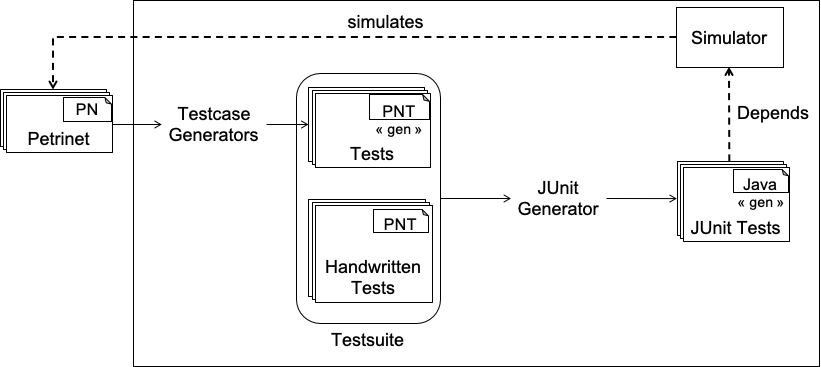
\includegraphics[scale=0.4]{src/pic/arch.png}
  \caption{The \emph{Petrinets Testing} language Architecture}
  \label{fig:arch}
\end{figure}

Based on the MontiCore Language Workbench \cite{monticore2020}, we propose the textual modeling language \emph{Petrinets Testing}. There are four main components in our \emph{Petrinets Testing} project, they are \emph{Testcase Generator}, \emph{Petrinets Testing language}, \emph{JUnit Test Generator} and \emph{Simulator}. The architecture of \emph{Petrinets Testing} project is in Fig \ref{fig:arch}. The specific responsibilities of each part are as follows:

\begin{itemize}
    \item \emph{Testcase Generator}: Any petri net model can be used as an input for the \emph{Petrinets Testing} project. First, we will use the \emph{petrinets4analysis} language to parse the given petri net model. Through the parsed petri net model, the system can automatically generate test cases using the algorithm we set, which will be mainly introduced in chapter \ref{sec:automatically generates testcase}. Furthermore, we can also create test cases manually according to the grammar of \emph{Petrinets Testing} language. Finally we will get a \emph{Petrinets Testing} model. \\
    
    \item \emph{Petrinets Testing language}: \emph{Petrinets Testing} is a domain-specific language (DSL) that is easily usable by domain experts without knowledge of programming. The grammar of the \emph{Petrinets Testing} language is defined by the MontiCore Language Workbench \cite{rumpe2017monticore}, which produces Java classes for the abstract syntax tree (AST) as well as additional infrastructure by our defined keywords and syntactic sugar in the MontiCore Language Workbench. In \emph{Petrinets Testing} language, we can define the initial markings, simulated transitions and expected markings of given petri net model. Each petri net model will have a corresponding \emph{Petrinets Testing} model (an example is in Listing \ref{lst:pnt-Cheap Cookie Machine}). Through the \emph{Petrinets Testing} language, we can define multiple test cases in the same model. \\
    
    \item \emph{JUnit Test Generator}: The petri net test needs to use JUnit, which is a simple framework to write repeatable tests, so the function of the {JUnit Test Generator} model is to convert the generated \emph{Petrinets Testing} model into a JUnit class. In each of JUnit class, we also add some auxiliary functions for the next simulation operation. \\
    
    \item \emph{Simulator}: After the program has generated \emph{Petrinets Testing} models for all petri nets, this module \emph{Simulator} will automatically execute the corresponding JUnit class for petri net testing. In the process of running, the program will first need the parsed petri net model of \emph{petrinets4analysis} language, so the \emph{petrinets4analysis} language is also used in this process. When the results of each JUnit class running meets the expected conditions, the system will finally give a "pass" signal.
\end{itemize}
% TeX root = ../../paper.tex

\section{Background}\label{sec:background}

We assume that the reader is familiar with the basic concept of a petri net. Nevertheless, we quickly introduce the fundamentals in this chapter. In addition, the \emph{Petrinets Testing} language can automatically create the testcase of given petri net model by cause-effect-net\cite{Desel1997}, so we also introduce the concept of cause-effect-net in this chapter.

\subsection{Petri Nets}\label{sec:background:definition}

Petri nets are a graphical and mathematical modeling tool which are useful for modeling systems with concurrent, asynchronous, distributed or parallel properties. They have been observed to have broad application in modeling finite state machines, parallel activities, dataflow computations, communication protocols, sychronization control, discrete event systems, and asynchronous circuits \cite{murata1989petri}. They were introduced by Carl Adam Petri in 1962 \cite{petri1962kommunikation}. In early 1970’s MIT was very active in the research of Petri nets. Since the late 1970’s, European researchers have organized workshops and published conference proceedings on Petri nets \cite{murata1989petri}.

The Petri nets can mathematically be described as follows:

Let $\mathbb{N}$ denote the set of nonnegative integers. A Petri net with inhibitor arcs is a 6-tuple $ PN = (P, T, F, I, V, m_0)$, where: 

\begin{itemize}
    \item $P=\{p_1, p_2, ... , p_{|P|} \}$ is a set of places, where $|P|$ denotes the cardinality of set $P$,
    \item $T = \{ t_1, t_2, ... , t_{|T|}\}$ is a set of transitions, where $|T|$ denotes the cardinality of set $T$ and $P \cap T = \emptyset $,
    \item $ F \subseteq (P \times T) \cup (T \times P)$,
    \item $ I \subseteq (P \times T)$,
    \item $V$ is a weight function: $F \rightarrow \mathbb{N}$, and
    \item $m_0$ is the the initial marking $P \rightarrow \mathbb{N}$.
\end{itemize}

Petri nets can be viewed as bipartite directed multigraphs. The set of nodes is divided into two disjoint sets: $P$ and $T$. An arc in $F$ connects a pair of nodes in $P \times T$ or $T \times P$. The mapping $V$ assigns non-negative integers to arcs. An arc assigned with number $k$ denotes $k$–parallel arcs between the same pair of nodes. A \emph{marking} $m \in (\mathbb{N} \cup 0)^n $ is a mapping from every place $p$ to a non-negative integer. If the number $k$ is assigned to the place $p$, we say that there are $k$ tokens on place $p$. The number of tokens on place $p$ under marking $m$ is represented by $m(p)$. The initial marking $m_0$ is the distribution of tokens between the places of the net before any action is taken. The input place of a transition $t$ , denoted as $t^−$ , is a set of places $\{ p | p \in P, (p, t) \in F \}$ . The output place of a transition $t$ is a set of places defined as $\{ p | p \in P, (t, p) \in F \}$ , and is denoted by $t^+$ . The functions $t^−(p) = i$ is defined as $(p, t) \in F$ and $V ((p, t)) = i$. Similarly $t^+(p) = i$ is defined as $(t, p) \in F$ and $V(t, p) = j$.

A transition $t$ is said to be enabled given a marking $m$ iff $\forall p \in t^− , m(p) \geq t^− (p)$. An enabled transition is ready to \emph{fire}. When a transition fires, it removes tokens from its input places and puts tokens in its output places. An enabled transition may or may not fire, and there may be more than one transition enabled in a given marking, but only one transition can fire at a time. If the current marking of the net is $m$, $t$ is the fired transition, and $m^\prime$ is the marking after the firing of $t$, the relation between $m$ and $m^\prime$ is $m^\prime (p) = m(p) − t^− (p) + t^+ (p)$, for every $p \in P$.

An inhibitor arc in $I$ is an arc connecting a place and a transition. The connected transition cannot fire if the input place along the inhibitor arc contains at least one token. A transition with inhibitor arcs is enabled iff $\forall p \in t^− , m(p) \geq t^− (p)$ and every input place along the inhibitor arcs contains no token. After the transition fires, no token is removed through the inhibitor arc. Inhibitor arcs give Petri nets the ability to test "zero". This extends the modeling power of Petri nets to the level of Turing machines.


\subsection{Cause Effect Net}

The cause-effect-net is evolved from cause-effect graphing, which is a method of a black box program testing. The cause-effect graphing \cite{srivastava2009cause} is used to describe the causal relationship between the input and output of the system, and the constraint relationship between the input and the output. The drawing process of the cause-effect graphing is the modeling process of the external characteristics of the tested system. According to the cause-effect graphing between the input and output of the system, the judgment table is also called the test case table, so as to plan the test case. The cause-effect-net also generates tables in the same way as cause-effect graphing. When we have the test case table, then we can generate the corresponding the \emph{Petrinets Testing} model according to the \emph{Petrinets Testing} language grammar. \\

There are four types of relationships in the Petri net that need to be considered, they are OR-, AND-, SINGLE- and ALTERNATE-relationship. According to these four types of relationships, we define the input places of transition as a cause or combination of causes, and the output places of transition as effects. The following are the definitions of the four relationships:

\begin{itemize}
    \item OR-relationship: \\ 
        Alternative causes which belong to the same effect (see Fig \ref{fig:OR-relationship})
    \item AND-relationship: \\ 
        Common causes which belong to one effect (see Fig \ref{fig:AND-relationship})
    \item SINGLE-relationship: \\ 
        A cause which directly leads to one effect (see Fig \ref{fig:SINGLE-relationship})
    \item ALTERNATE-relationship: \\
        A single cause or a combination of causes may lead to different effects (see Fig \ref{fig:ALTERNATE-relationship})
\end{itemize}

\begin{figure}
\centering
\begin{minipage}{.5\textwidth}
  \centering
  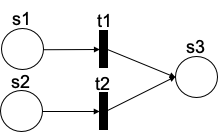
\includegraphics[width=.8\linewidth]{src/pic/OR.png}
  \captionof{figure}{OR-relationship}
  \label{fig:OR-relationship}
\end{minipage}%
\begin{minipage}{.5\textwidth}
  \centering
  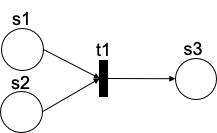
\includegraphics[width=.8\linewidth]{src/pic/AND.png}
  \captionof{figure}{AND-relationship}
  \label{fig:AND-relationship}
\end{minipage}
\end{figure}

\begin{figure}
\centering
\begin{minipage}{.5\textwidth}
  \centering
  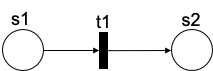
\includegraphics[width=.8\linewidth]{src/pic/SINGLE.png}
  \captionof{figure}{SINGLE-relationship}
  \label{fig:SINGLE-relationship}
\end{minipage}%
\begin{minipage}{.5\textwidth}
  \centering
  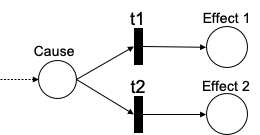
\includegraphics[width=.9\linewidth]{src/pic/ALTERNATE.png}
  \captionof{figure}{ALTERNATE-relationship}
  \label{fig:ALTERNATE-relationship}
\end{minipage}
\end{figure}

The most important of the four types of relationship is the ALTERNATE-relationship, because this is a non-determinism relationship, which means the place has more than one successor transition. In our algorithm, we focus on finding the ALTERNATE-relationship in the all Petri net to determine the causes and effects in the cause-effect-net.





% TeX root = ../../paper.tex

\section{Language}\label{sec:language}

The grammar is the foundation of the \emph{Petrinets Testing} language which is defined on a syntactical level and on a semantic level, both aided by MontiCore generation capabilities.

\subsection{Grammar Design}

The syntactic foundation of the \emph{Petrinets Testing} language is a context-free grammar which defines all valid keywords and permissible input values as well as syntactic sugar (e.g. punctuation and bracketing), and their static arrangement~\cite{rumpe2017monticore}. The grammar of the \emph{Petrinets Testing} language (see Listing \ref{lst:language:grammar}) is defined by the MontiCore Language Workbench, which produces Java classes for the abstract syntax tree (AST) as well as additional infrastructure by our defined keywords and syntactic sugar in the MontiCore Language Workbench. The desired modeling elements are

\begin{itemize}
    \item Testcase features: orginal petri net, testcase body, testing step, testing expectation
    \item Testcase body elements: initial markings, inherit markings, define markings, markings with places
    \item Testing step elements: defined simulation
    \item Testing expectation elements: place binding with any or all conditional markings
\end{itemize}

\begin{lstfloat}
	\centering
\begin{lstlisting}[style=mcgrammar]
grammar PetrinetTests extends de.monticore.literals.MCCommonLiterals  {

    symbol scope PetriNetTest = "pntest" Name "{"
        Import
        (TestcaseBody | Testcase+)
    "}";

    symbol Testcase = "testcase" Name "{"
        TestcaseBody
    "}";

    Import = "use" "petrinet" Name;

    TestcaseBody = InitialMarking Expectation* TestStep*;
    TestStep = Simulation+ Expectation+;
    Simulation = "simulate" "{" (Name || ",")+ "}";

    InitialMarking = "initial" "marking" (InheritMarking | DefineMarking);
    InheritMarking = "inherited" RestSpecification?;
    DefineMarking = "{" (PlaceBinding || ",")* ("," RestSpecification)? "}";
    PlaceBinding = place:Name value:MarkingValue;
    RestSpecification = "rest" MarkingValue;
    MarkingValue = NatLiteral;

    Expectation = "expect" Condition;
    interface Condition;
    astrule Condition = 
      method Optional<Boolean> verify(
        petrinet._ast.ASTPetrinet petrinet, petrinet.analysis.Marking marking) { };
    interface BooleanCondition extends Condition;
    Negation implements BooleanCondition = "not" Condition;
    Conjunction implements BooleanCondition = "all" "{" (Condition || ",")* "}";
    Disjunction implements BooleanCondition = "any" "{" (Condition || ",")* "}";

    MarkingCondition implements Condition = 
      "marking" "{" (PlaceBinding || ",")* "}";
    EnabledCondition implements Condition = 
      "enabled" "{" (Name || ",")* "}";
}
\end{lstlisting}
	\caption{The \emph{Petrinets Testing} MontiCore grammar}\label{lst:language:grammar}
\end{lstfloat}


The \textbf{PetriNetTest} grammar defines the structure of the \emph{Petrinets Testing} language. Firstly, the grammar should know which petri net needs to be tested, so we define \textbf{Import}, which is to import the original petri net model that needs to be tested, which is parsed by the \emph{petrinets4analysis} language\cite{Hein}. The following part is about the all testcases of the original petri net model. The \textbf{PetriNetTest} grammar can contain one and more than one one-terminal \textbf{Testcase}. In each testcase body, we can define the \textbf{InitialMarking} of the petri net that needs to be tested. If we want to use the initial markings from the original petri net model, we can use the \textbf{InheritMarking} to inherit the original markings. Moreover, we can also make modifications to the inherited markings. If we want to define the new initial markings, we can use \textbf{DefineMarking} non-terminals to define the initial markings we need, which can be specified in their corresponding places.

In the testing step part, we can use \textbf{Simulation} non-terminals to specify which transitions are required for the \emph{Petrinets Testing} language model to simulate, where the order of the transitions affects the final testing expectation.

In the testing expectation part, we can use \textbf{Expectation} to define the expected markings model will reach, which can be specified in their corresponding places. In order to realize the conditional expected markings, we define \textbf{BooleanCondition} interface utilizing MontiCore through an \textbf{astrule} \textbf{Condition} for the \textbf{Expectation} non-terminal. At this point we can define various combinations of expected markings with "all" and "any" keywords.

\subsection{Well-formedness of Models}\label{sec:lang:semantics}

The grammar ensures syntactic correctness of the \emph{Petrinets Testing} model definitions, but additionally, models must be well-formed. Context conditions (CoCos) in MontiCore are used to verify the semantic correctness of the \emph{Petrinets Testing} model. A context condition is a predicate on a context-free grammar correct sentence where the context of a word is used to determine the total correctness, also called well-formedness\cite{rumpe2017monticore}. 

The \emph{Petrinets Testing} language uses the \emph{petrinets4analysis} language to parse the petri net model, and the \emph{Petrinets Testing} language will simulate the petri net with the defined initial markings and transitions, so a place that appears in the \emph{Petrinets Testing} model must exist in the petri net model in the \emph{petrinets4analysis} language. In addition, all transitions in the \emph{Petrinets Testing} model must also exist in the petri net model in the \emph{petrinets4analysis} language.
% TeX root = ../../paper.tex

\section{Automatic Test Case Generation}\label{sec:automatically generates testcase}
\label{sec:generation}

The \emph{Petrinets Testing} language can automatically analyze the Petri net and automatically generate test cases of this petri net. We decided to use cause-effect-net \cite{Desel1997} to automatically create test cases. In this paper \cite{Desel1997}, the author introduced how to find Causes and Effects, and provided a method to create a casue-effect-net to generate a test case table. We adopt the method mentioned in the paper and implement it with a program to complete the automatic generation of the test case table about a given petri net.

\subsection{Test case generation}
We use the \emph{petrinets4analysis} language to parse the given Petri net and obtain the entire Petri net, and then use the algorithm to transform the Petri net into the cause-effect-net and get the test case table. \\

\begin{itemize}
    \item Step 1: Finding the causes and effects: \\
    First, finding all ALTERNATE-relationships in the given Petri net and recording the corresponding transitions. These transitions are the all non-determinism transition in the original Petri net and will be all transitions in the cause-effect-net. \\
    
    \item Step 2: Linking the causes and effects: \\
    Then analyzing all input places corresponding to these transitions using the OR-, AND-, SINGLE- and ALTERNATE-relationship and recording them. These associated input places are the causes. In addition, analyzing all output places corresponding to these transitions using the OR-, AND-, SINGLE- and ALTERNATE-relationship and recording them. These associated output places are the effects. \\
    
    \item Step 3: Generating cause-effect-net: \\
    According to the recorded transitions and the corresponding input and output places, a cause-effect-net of this Petri net can be created, which is similar to the generation of the Boolean graph. \\
    
    \item Step 4: Generating test case table: \\
    According to the generated cause-effect-net, each column in the test case table corresponds to a transition, and each row corresponds to the input and output places. When a transition has input and output places, the corresponding grid is marked as one.\\
    
    \item Step 5: Generating \emph{Petrinets Testing} model: \\
    According to the generated test case table, the simple transition test case model can be generated by the \emph{Petrinets Testing} language using PrettyPrinter. The test case model will be saved in the form of a file in the designated location to provide support for the next generating test code step.
    
\end{itemize}

\subsection{Example}
An specific example for the automatic test case generation from a Petri net, which is a simplified workflow of a cheap cookies machine (see Fig \ref{fig:cheap-cookie-machine}) with the following transitions:

First, coin is put into the cookies machine and will be checked whether is accepted. If the coin is accepted and the cookies button is pressed, the machine will receive the signal and give the cookies. At the same time, the amount of the cookies store and the number of cookies counter will be reduced. The machine will not accept a new signal until the money is cleared. \\

\begin{figure}
  \centering
  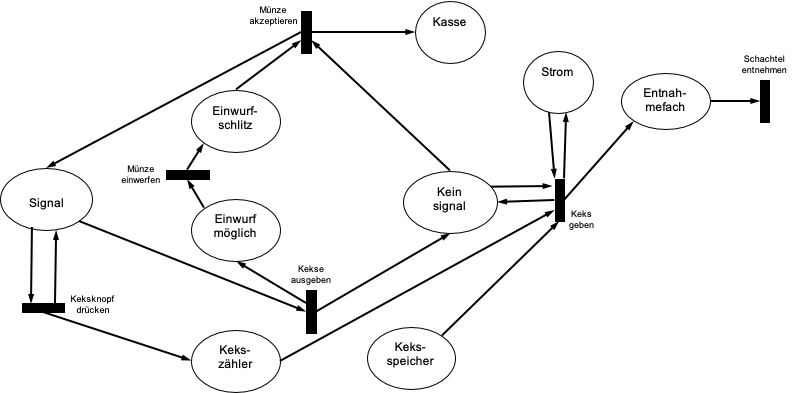
\includegraphics[scale=0.45]{src/pic/cheap-cookie-machine.png}
  \caption{Petri Net: Cheap Cookie Machine \cite{Hein}}
  \label{fig:cheap-cookie-machine}
\end{figure}

\subsubsection{Finding the causes and effects}
Firstly, we traverse all transitions in order to search all ALTERNATE-relationships in this Petri net. So we can find two places and four transitions that they meet the ALTERNATE-relationship conditions. They are \emph{Signal} places with \emph{Keksknopf drücken} and \emph{Kekse ausgeben} transitions, and \emph{Keinsignal} with \emph{Münze akzeptieren} and \emph{Keks geben} transitions. Then we record these four transitions into a temporary table.

\subsubsection{Linking the causes and effects}
Secondly, we analyze all input and output places about these four transitions using the OR-, AND-, SINGLE- and ALTERNATE-relationship and record them into a temporary table. The following is the temporary table about recorded transitions and input and output places:

\begin{enumerate}
    \item Transition: \emph{Keks drücken}
    \begin{itemize}
        \item Input places: \emph{Signal}
        \item Output places: \emph{Signal}, \emph{Kekszähler}
    \end{itemize}
    \item Transition: \emph{Kekse ausgeben}
    \begin{itemize}
        \item Input places: \emph{Signal}
        \item Output places: \emph{Einwurfmöglich}, \emph{Keinsignal}
    \end{itemize}
    \item Transition: \emph{Keks geben}
    \begin{itemize}
        \item Input places: \emph{Kekszähler}, \emph{Keksspeicher}, \emph{Strom}, \emph{Keinsignal}
        \item Output places: \emph{Keinsignal}, \emph{Entnahmefach}, \emph{Strom}
    \end{itemize}
    \item Transition: \emph{Münze akzeptieren}
    \begin{itemize}
        \item Input places: \emph{Keinsignal}, \emph{Einwurfschlitz}
        \item Output places: \emph{Kasse}
    \end{itemize}
\end{enumerate}

\subsubsection{Generating cause-effect-net}
According to the temporary table above, we can create a cause-effect-net (see Fig \ref{fig:cause-effect-net}) of the original Petri net. At the same time, we mark transition \emph{Keks drücken} as 1, taransition \emph{Kekse ausgeben} as 2, transition \emph{Keks geben} as 3 and transition \emph{Münze akzeptieren} as 4 for the convenience of generating test case table.

\begin{figure}
  \centering
  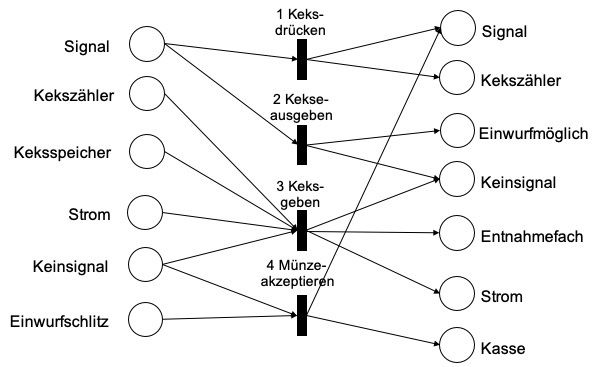
\includegraphics[scale=0.5]{src/pic/cause-effect-net.png}
  \caption{cause-effect-net of Cheap Cookie Machine model}
  \label{fig:cause-effect-net}
\end{figure}

\subsubsection{Generating test case table}
According to the cause-effect-net above, we can create a test case table (see Table \ref{tab:test-case-table}). In this table, we use the previously marked numbers 1,2,3,4 to represent transitions. In addition, Causes (Input places) and Effects (Output places) are distinguished. For example, we mainly focus on the third column in the table and the number 3 on the header stands for transition \emph{Keks geben}. Because \emph{Kekszähler}, \emph{Keksspeicher}, \emph{Strom}, \emph{Keinsignal} are the input places of transition \emph{Keks geben}, all corresponding positions in Causes are marked as 1. Similarly, \emph{Keinsignal}, \emph{Entnahmefach}, \emph{Strom} are the output places of transition \emph{Keks geben}, so all corresponding positions in Effects are marked as 1. Other transitions are marked by analogy. Finally we get a complete test case table about Petri net "Cheap Cookies Machine".

\begin{table}[]
    \centering
    \caption{Test case table of Cheap Cookie Machine model}
    \label{tab:test-case-table}
    \begin{tabular}{|p{3cm}|p{.5cm}<{\centering}|p{.5cm}<{\centering}|p{.5cm}<{\centering}|p{.5cm}<{\centering}|}
        \hline
        \rowcolor{gray} 
        \textbf{TestCase}   & 1  & 2  & 3  & 4  \\ \hline
        \multicolumn{5}{|l|}{\textbf{Causes:}}  \\ \hline
        Signal              & 1  & 1  & 0  & 0  \\ \hline
        Kekszähler          & 0  & 0  & 1  & 0  \\ \hline
        Keksspeicher        & 0  & 0  & 1  & 0  \\ \hline
        Strom               & 0  & 0  & 1  & 0  \\ \hline
        Keinsignal          & 0  & 0  & 1  & 1  \\ \hline
        Einwurfschlitz      & 0  & 0  & 0  & 1  \\ \hline
        \multicolumn{5}{|l|}{}                  \\ \hline
        \multicolumn{5}{|l|}{\textbf{Effects:}} \\ \hline
        Signal              & 1  & 0  & 0  & 1  \\ \hline
        Kekszähler          & 1  & 0  & 0  & 0  \\ \hline
        Einwurfmöglich      & 0  & 1  & 0  & 0  \\ \hline
        Keinsignal          & 0  & 1  & 1  & 0  \\ \hline
        Entnahmefach        & 0  & 0  & 1  & 0  \\ \hline
        Strom               & 0  & 0  & 1  & 0  \\ \hline
        Kasse               & 0  & 0  & 0  & 1  \\ \hline
    \end{tabular}
\end{table}

\subsubsection{Generating \emph{Petrinets Testing} model}
According to the test case table above, the program can automatically generate a \emph{Petrinets Testing} model about transition test. Each column in the test case table will generate a testcase in the \emph{Petrinets Testing} model. The corresponding Causes in the table will be used as \emph{initial marking} in the model. Moreover, the corresponding Effects in the table will be used as \emph{expect marking} in the model and the transition will be used as \emph{simulate} in the model. Then the program uses the PrettyPrinter of the \emph{Petrinets Testing} language to write the model into a file (see Listing \ref{lst:pnt-Cheap Cookie Machine}).

\begin{lstfloat}
	\centering
    \begin{lstlisting}[style=mcgrammar]
pntest CookieMachine_AutoTest { 
    use petrinet CookieMachine_modified
    testcase KeksGeben_TransitionTest {
        initial marking {
            KeksZaehler 1,
            Keksspeicher 1,
            KeinSignal 1,
            Strom 1
        }
        simulate {
            KeksGeben
        }
        expect marking {
            KeinSignal 1,
            Entnahmefach 1,
            Strom 1
        }
    }
    ...
}
    \end{lstlisting}
	\caption{The \emph{Petrinets Testing} model of Cheap Cookie Machine model}
	\label{lst:pnt-Cheap Cookie Machine}
\end{lstfloat}
\input{src/tex/08.related work}
% TeX root = ../../paper.tex
%
\section{Implementation}\label{sec:implementation}


The base of the \emph{Petrinets Testing} language is the MontiCore Language Workbench~\cite{rumpe2017monticore} 6.1.0 which is a fully featured framework for the development of domain-specific languages. Based on the grammar that we present above, it is able to generate, among many other tools, a parser for models that conform to the grammar which also translates the model to a powerful and easy to manipulate data structure, the Abstract Syntax Tree (AST).
As code is generated even before compile time it also provides a development infrastructure that is specifically suited to work with our DSL and is easy to extend with more features, including code generation.
This also means that only the parts that specifically concern the functionality of the language models had to be implemented.

We use unit testing to evaluate our implementation, aiming for a high degree of test coverage.


\begin{figure}
  \centering
  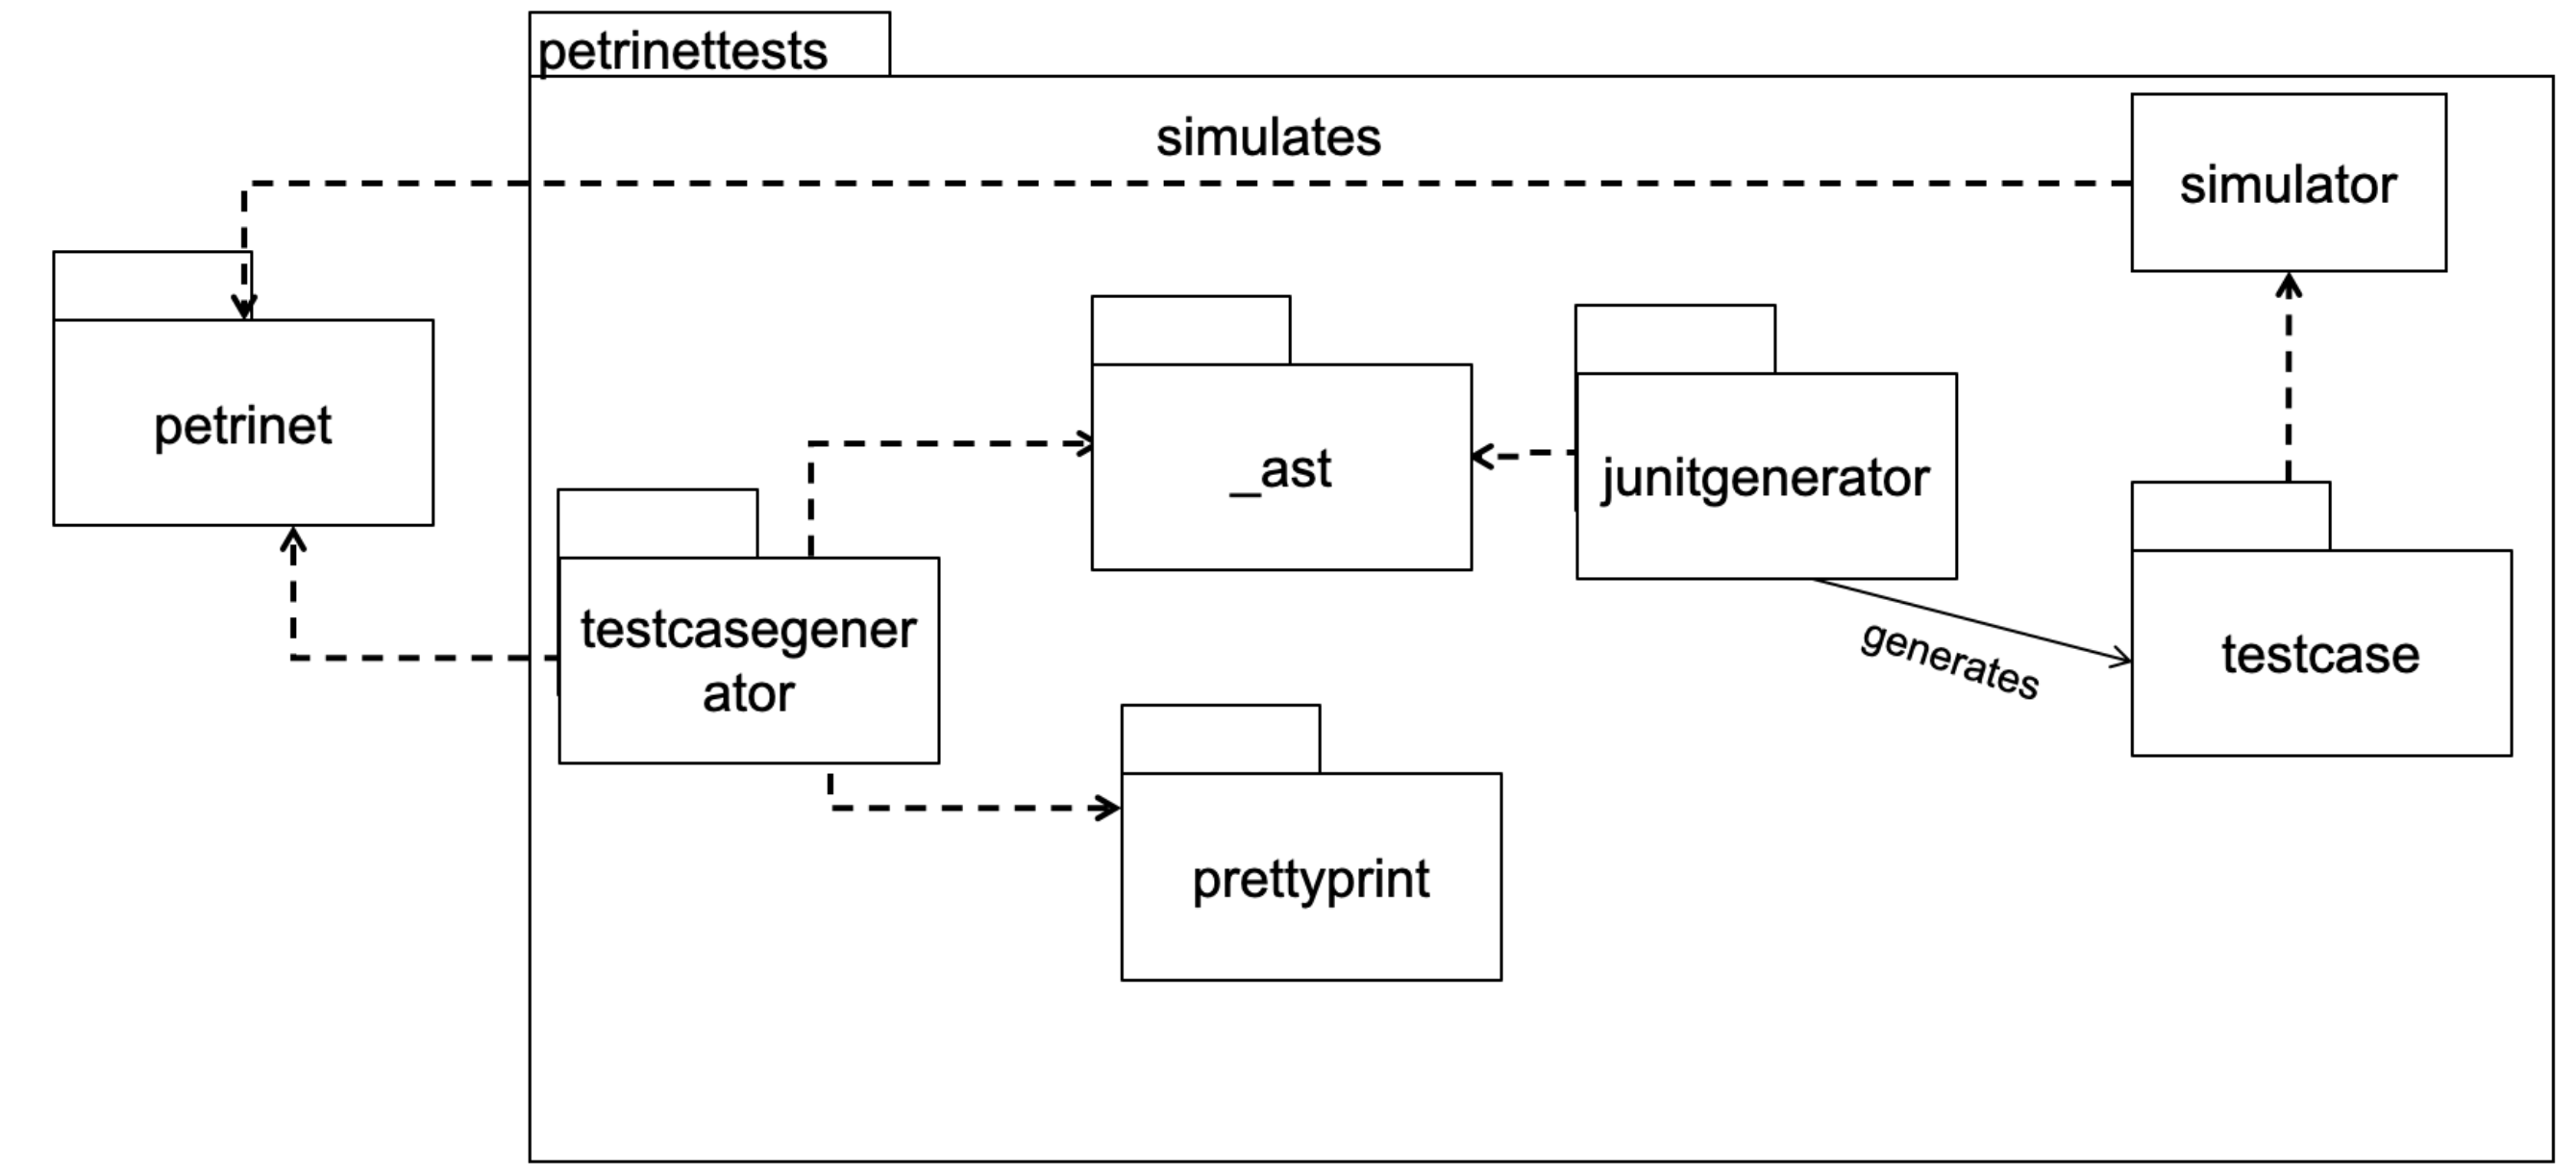
\includegraphics[width=\textwidth]{src/pic/architecture.png}
  \caption{The \emph{Petrinets Testing} language Architecture}
  \label{fig:architecture}
\end{figure}


Figure \ref{fig:architecture} shows the top-level architecture based on packages as well as their interactions. \textbf{petrinet} here stands for the \emph{petrinet4analysis} language. In the following, we describe the main roles of the individual packages.


\begin{itemize}
	\item \textbf{testcasegenerator} contains the classes that implement the automatic generation of test cases based on models provided as \emph{petrinet4analysis} AST. The mechanism that is implemented here is explained in detail in \ref{sec:generation}.
	\item \textbf{prettyprint} Using the PrettyPrinter, it is possible to inspect a \emph{Petrinet Testing} model by printing it to a string. It makes use of the IndentPrinter provided by MontiCore, as well as the Visitor pattern. Its main use case is the export of ASTs that have been generated by the \textbf{testcasegenerator} package.
	\item \textbf{junitgenerator} provides functionality of generating executable testcases from \textit{Petrinet Testing} models. This makes use of the MontiCore support for generation. Several templates are defined in the \textit{FreeMarker} template language and passed to MontiCore along with the AST to generate from. This results in Java code that implements a JUnit test case.
	\item \textbf{simulator} could be seen as a run-time environment for generated test cases. The generated test cases require on this package which is able to perform operations on \emph{petrinet4analysis} ASTs needed to perform the individual test steps. This includes setting a marking on a petri net and updating the marking based on transitions.
\end{itemize}

\subsubsection{Tool} In additon to that, we provide a command line interface as a user interface to our toolset. It supports both the generation of \textit{Petrinet Testing} models from \textit{petrinet4analysis} models using the \textbf{testcasegenerator} package, as well as the generation of JUnit tests from \textit{Petrinet Testing} models. The tool is accessible through the command \texttt{java -jar petrinet-tests.jar}, where the file petrinet-tests.jar has to be the fully assembled jar file. The \texttt{--help} flag provides user information about the tool.

\subsubsection{Running tests}
We provide a separate maven module \textit{petrinet-tests-runner} that is able to parse models and execute all defined tests automatically. Both \textit{petrinet4analysis} and \textit{Petrinet Testing} models can be placed in to the module's \texttt{src/main/resources} directory to be considered. The generated files will be stored in the directory \texttt{target/generated-test-sources}.

This process is already included in the standard maven build process and can therefore be triggered by running \texttt{mvn install}.

\subsubsection{Workflow}
A workflow that combines several use cases of our toolset could therefore look as follows.
First, the user defines the model they wish to test as a \emph{petrinet4analysis} model. Along with that, they can define hand-written test cases and write them using \textit{Petrinet Testing} models.
Then, using the PetrinetTestsTool, they can trigger the automatic generation of testcases described in section \ref{sec:generation}. This will generate additional \textit{Petrinet Testing} model files. 
Both the \textit{petrinet4analyis} and the \textit{Petrinet Testing} models can be placed into the folder mentioned above. By running the maven goal install, the run of the runner module described above is triggered. It reads all defined models and generates executable JUnit tests that execute the defined test cases. As the tests are directly run, the user is able to read the test results directly from the console.

\subsection{Adaptations to \emph{petrinet4analysis}}

In order to be compatible with \textit{petrinet4analysis}, a few adaptions to that implementation were required which are described in this section.

The \emph{Petrinets Testing} language is supplemented by the grammar in \emph{petrinets4analysis} language \cite{Hein}. The \emph{Petrinets Testing} language uses MontiCore 6.1.0 \cite{monticore2020} to establish the project, but the \emph{petrinets4analysis} language used the version of MontiCore was 5.0.3 \cite{rumpe2017monticore}. In order to better use the grammar in \emph{petrinets4analysis} language and seamlessly connect with our project, we decided to upgrade the MontiCore version used by \emph{petrinets4analysis} language.


The \emph{petrinets4analysis} language used MontiCore 5.0.3 to create the grammar language and implement the project. There are some differences between MontiCore 5 and MontiCore 6. In MontiCore, all grammars are dependent on the most basic grammar class, which is \emph{de.monticore.literals.Literals} in MontiCore 5.0.3 but \emph{de.monticore.literals.MCCommonLiterals} in MontiCore 6.1.0. There are all differences of \emph{petrinets4analysis} language in MontiCore 5.0.3 and MontiCore 6.1.0 in Table \ref{tab:diff-table}

\begin{table}
  \begin{threeparttable}
    \caption{Differences of \emph{petrinets4analysis} language in MontiCore 5.0.3 and MontiCore 6.1.0}
    \label{tab:diff-table}
     \begin{tabular}{|c|l|l|}
        \hline
        \multicolumn{1}{|l|}{} & \multicolumn{1}{c|}{MontiCore 5.0.3} & \multicolumn{1}{c|}{MontiCore 6.1.0}     \\ \hline
        \multirow{2}{*}{MC4}    & de.monticore.literals.Literals       & de.monticore.literals.MCCommonLiterals   \\ \cline{2-3} 
                              & IntLiteral                 & NatLiteral                          \\ \hline
        \multirow{4}{*}{Java} & Scope                      & PetrinetArtifactScope               \\ \cline{2-3} 
                              & GlobalScope                & PetrinetGlobalScope                 \\ \cline{2-3} 
                              & PetrinetSymbolTableCreator & PetrinetSymbolTableCreatorDelegator \\ \cline{2-3} 
                              & ResolvedSeveralEntriesException      & ResolvedSeveralEntriesForSymbolException \\ \hline
    \end{tabular}
    \begin{tablenotes}
      \small
      \item Note: MC4 is the filename extension of grammar file and Java is the filename extension of java file.
    \end{tablenotes}
  \end{threeparttable}
\end{table}

In the \emph{petrinets4analysis} language upgrade, one of the difficulties is the definition of the number type. According to \emph{de.monticore.literals.Literals} in MontiCore 5.0.3, the \emph{petrinets4analysis} language used \emph{IntLiteral} to define number type, but in \emph{de.monticore.literals.MCCommonLiterals} of MontiCore 6.1.0, the \emph{IntLiteral} is no longer used. Therefore we analyzed the role of \emph{IntLiteral} in the \emph{petrinets4analysis} language project, and finally we decided to replace it with \emph{NatLiteral} in MontiCore 6.1.0. The return of getValue method of \emph{IntLiteral} in MontiCore 5.0.3 is Optinal class in Java 8, but the return of getValue method of \emph{NatLiteral} in MontiCore 6.1.0 is normal Int class, so we changed the corresponding algorithm logic in the place about \emph{NatLiteral} in MontiCore 6.1.0. \\

In addition, another thing worth paying attention to during the upgrade is scope. The naming method of Scope and GlobalScope are different in the automatically generated code of MontiCore 5.0.3 and MontiCore 6.1.0. For example, Scope in the \emph{petrinets4analysis} language of MontiCore 6.1.0 is PetrinetArtifactScope and GlobalScope is PetrinetGlobalScope. Moreover, we also made corresponding changes to the remaining related code about symbol table and exception handling.


\subsection{Extensibility and Future Work}

Many aspects of our design consider the need for future extensibility. 

Many more advanced techniques of generated test cases exist that take into account different coverage criteria. In the future, they can be implemented by adding new algorithms to the \textbf{testcasegeneration} package.

Also, by swapping out the implementation of the \textbf{simulator} package, it would be possible to not only perform tests on \textit{petrinet4analysis} models but to provide an actual system to test.

% TeX root = ../../paper.tex

\section{Conclusion}

Petri nets provide a versatile tool for modeling processes.
We further extended the petri net description language \emph{petrinets4analysis} to comply to the current version of the MontiCore  Language Workbench and on that basis developed a specific language, \emph{Petrinets Testing} to model test cases on such petri nets.
In addition we added capabilities for automated test case generation and provided an implementation for a generator utilizing cause effect nets.

The \emph{Petrinets Testing} language offers a simple and concise yet powerful way of specifying deterministic test cases. Each of which is tested by simulating the referenced petrinet by firing the specified transitions in the correct order and asserting that the defined properties hold.
By only focusing on necessary language constructs this enables others to create handwritten tests in order to check specific properties on a petrinet.

With the provided petri net simulation-interfaces we enable future developers to plug in their own implementations to be simulated as described in the test cases. Together with interfaces for automatic test case generators this creates an extensible framework which can be used to automatically apply the desired tests on the actual processes, modelled by the petri net.

The MontiCore Language Workbench \cite{rumpe2017monticore} played a major role in developing this framework.
It enabled us to focus on language design and tool-functionality by automatically generating all necessary steps to parse, verify and transform a language. Only a minimal additional codebase was needed to connect the two languages to work in unison.
Leveraging these capabilities, other developers will also benefit from the consistent and easy to understand interface , which in turn further adds to the extensibility of the overall framework.


\bibliography{src/bib/Literatur.bib}
\bibliographystyle{lncs/splncs04}

\end{document}